La caracterización de las propiedades de los muones es parte importante de este estudio, obtener las dependencias empíricas entre ellas y los posibles cambios en los límites de estas propiedades resultado del cambio de la eficiencia de los detectores en sus diferentes configuraciones se hace necesario para comprender mejor como se visualiza la teoría investigada desde su reconstrucción por los detectores.



Ante la necesidad de hacer estadística con las variables $\chi$ definimos la frecuencia de cada una de estas variables $\mathbb{F}_\chi^{(\mathtt{k})}$(x) donde para un valor predefinido de resolución de la información $\delta \chi$
\begin{equation}
\mathtt{\Theta(X,~Y)} ~ = ~ \Bigg\{\begin{matrix}
1 & \mathtt{X-\Delta X ~<~Y ~and~Y~ < X+\Delta X}\\
0 & \mathtt{X-\Delta X ~>~Y ~~or~~Y~ > X+\Delta X}
\end{matrix} 
\end{equation}

\begin{equation}
\mathbb{F}_\chi^{(\mathtt{k})} (x)= \sum_{ji} \mathtt{\Theta}(\chi_i^{(j,k)},~x)
\end{equation}

\begin{equation}
f_\chi^{(\mathtt{k})} (x)= \mathbb{F}_\chi^{(\mathtt{k})} (x)/ \sum_x \mathbb{F}_\chi^{(\mathtt{k})} (x)
\end{equation}


%\texttt{MNeuL}, \texttt{MNeuD}, \texttt{MPhoD}, \texttt{TcPhoD})

\subsubsection{Momento transversal.}
En los gráficos superiores de la Fig. \ref{procesos_darksusy_PTyISO} se puede observar los valores de momento angular de todos los muones reconstruidos para eventos $\mathbb{E}_i^{(4\mu,~\mathtt{CMS})}$ (configuración \texttt{Run-2}) y $\mathbb{E}_i^{(4\mu,~\mathtt{HL})}$ (configuración en \texttt{High Luminosity}), en estos se puede visualizar las diferencias entre los rangos de detección donde para eventos $k=$\texttt{CMS} el $\backsim ~ 99\%$ de los muones poseen $\sim 10  < ~ P_t^{(4\mu,~\mathtt{CMS})} ~ <\sim 100$, en contraste para $k=$\texttt{HL} tenemos $\sim 0.1 < ~ P_t^{(4\mu,~\mathtt{HL})} ~ < \sim 100$. Este aumento de rango en \texttt{HL} para valores menores de $\backsim ~ 10~GeV$ se puede ver que no es sin pérdidas, se puede constatar un cambio en la forma de los gráficos, esto es debido a que la inclusión de nuevos sensores en la configuración \texttt{HL} no poseen la misma eficiencia en la reconstrucción de la información.

\begin{figure}[!ht]
\centering
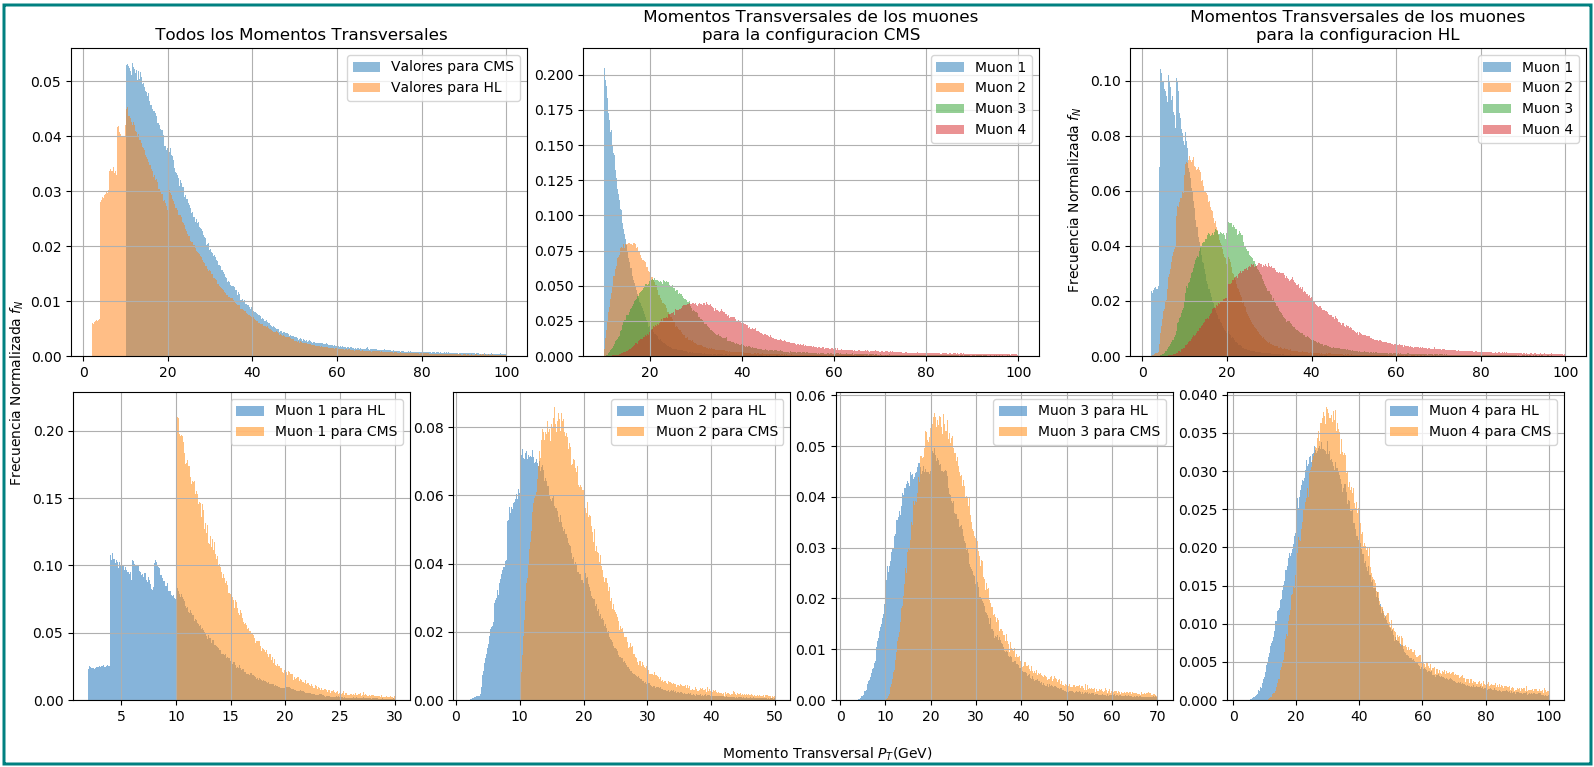
\includegraphics[width=.8\textwidth]{Simulacion/imagenes/Datos_PT_ALL.png}
%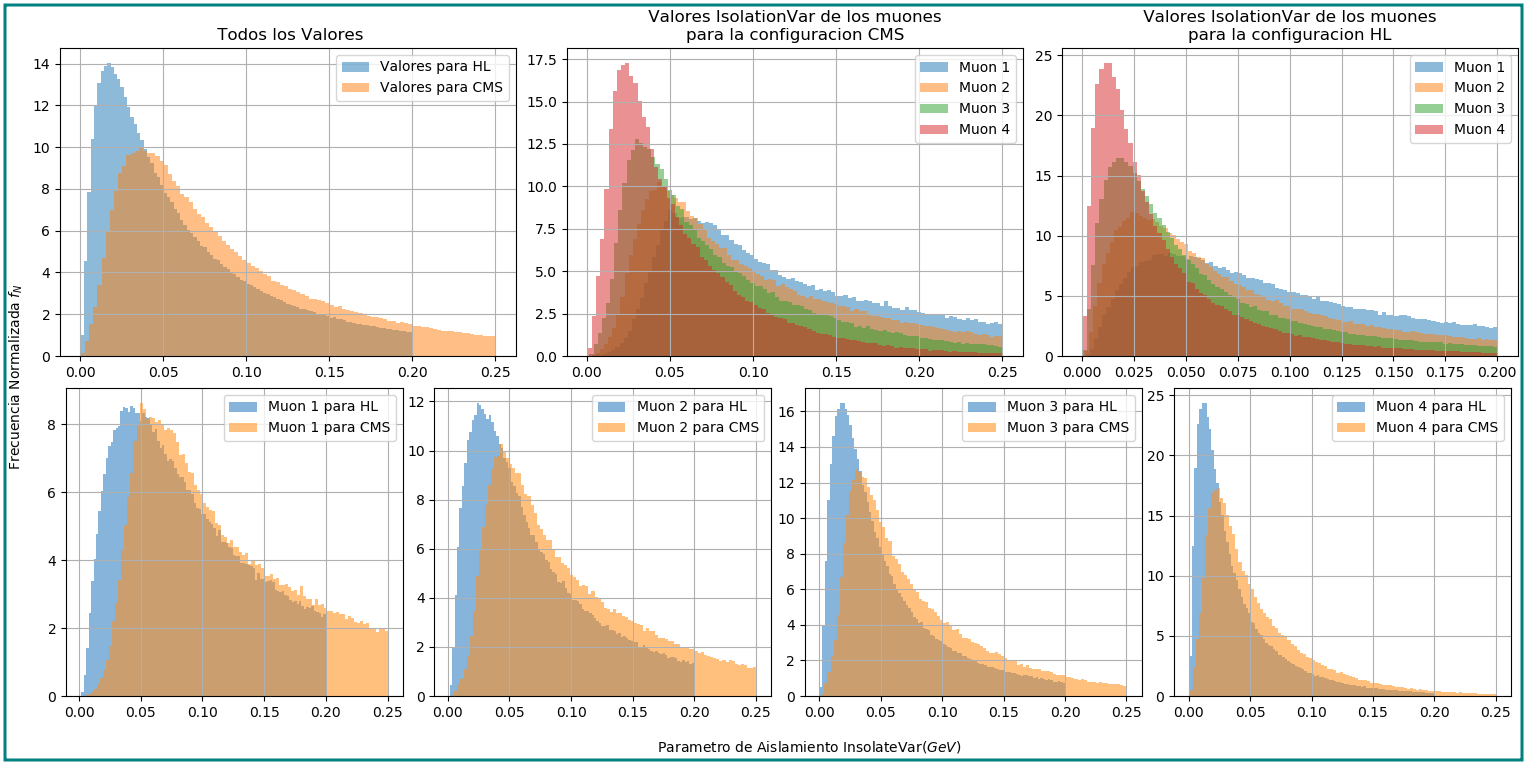
\includegraphics[width=.8\textwidth]{Simulacion/imagenes/Datos_IsolationVar_ALL.png}
\caption{Caracterización global de los momentos transversales de nuestra población de muones reconstruidos.}
\label{procesos_darksusy_PTyISO}
\end{figure}



\subsubsection{Valores de angulo}
\begin{figure}[!ht]
\centering
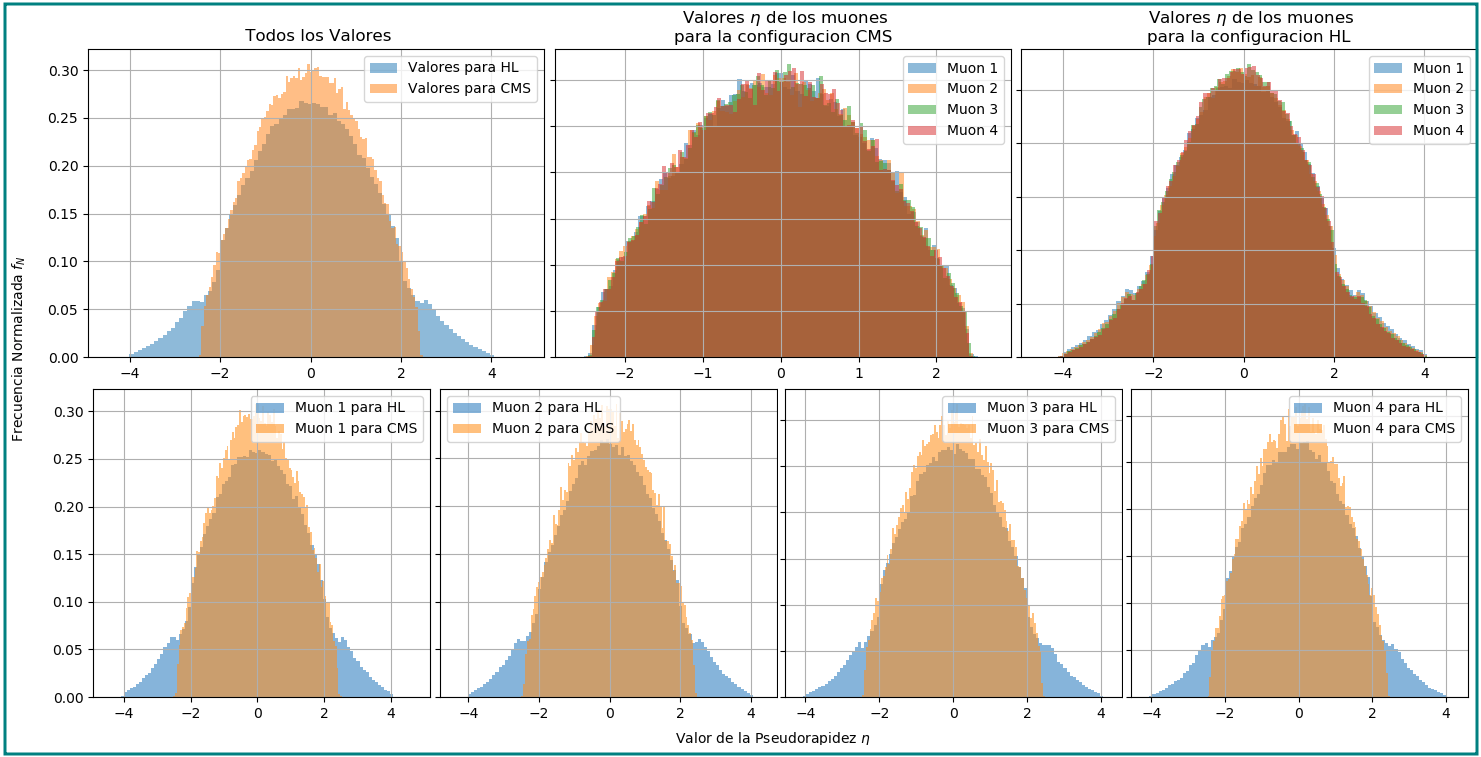
\includegraphics[width=.8\textwidth]{Simulacion/imagenes/Datos_Eta_ALL.png}
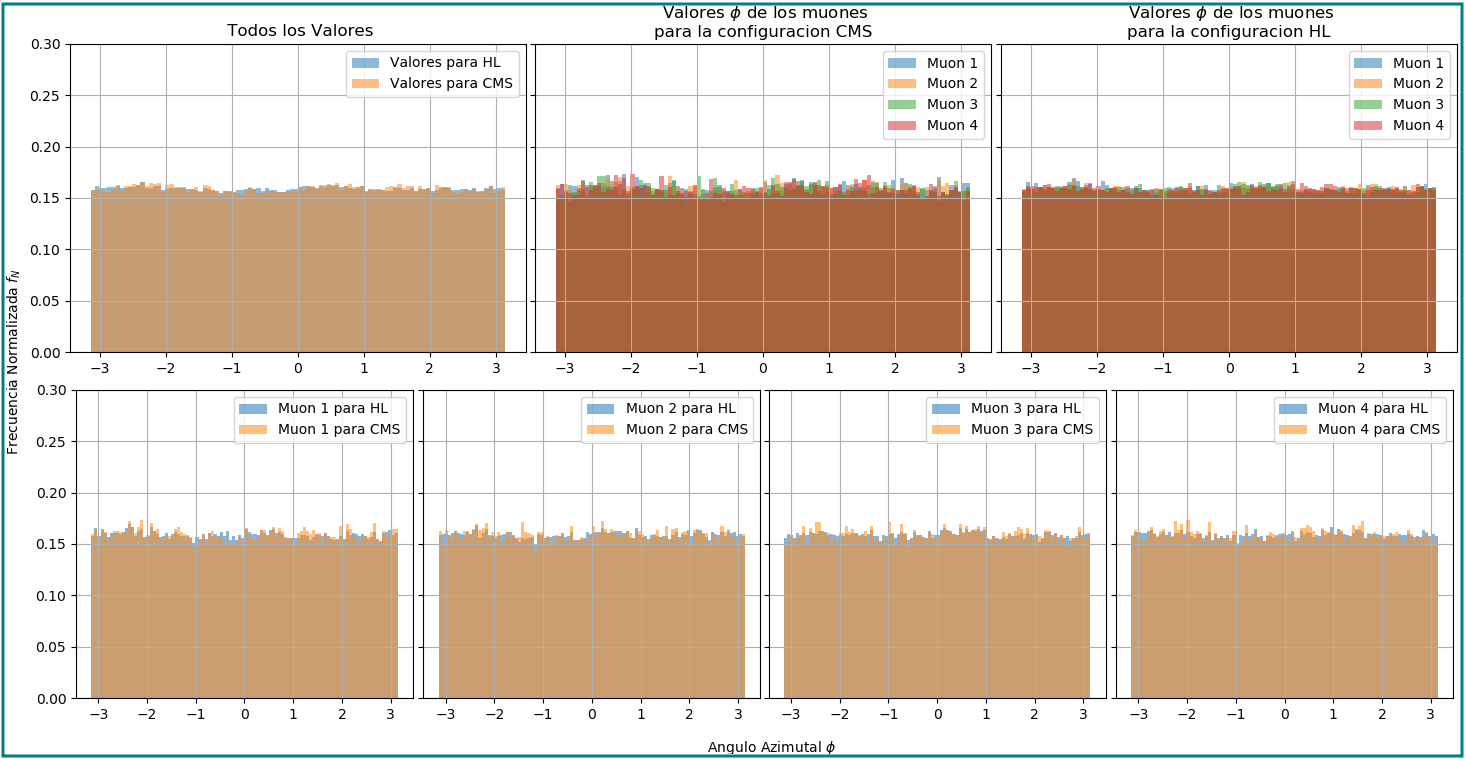
\includegraphics[width=.8\textwidth]{Simulacion/imagenes/Datos_Phi_ALL.png}
\caption{Grupo total de datos generados para los eventos de interes.}
\label{procesos_darksusy_ETAyPHI}
\end{figure}





Otro factor importante en la detección de los muones es el valor de Entonces de forma generar se puede Además como límite superior se puede constatar que el  se encuentran para valores 



















